                 % Chapter Template

\chapter{Situation Assessment} % Main chapter title

\label{chap-situation_assessment} % Change X to a consecutive number; for referencing this chapter elsewhere, use \ref{ChapterX}

\lhead{Chapter . \emph{Situation Assessment}} % Change X to a consecutive number; this is for the header on each page - perhaps a shortened title

In this chapter we introduce the Situation Assessment capacities of our system. Section \ref{sec:situation_assessemnt-intro} provides an introduction to the subject, with a discussion on some relevant works. Section\ref{sec:situation_assessment-overview} shows an overview of this layer, discussing its key aspects and modules. Sections \ref{sec:situation_assessment-object_human_detection} and \ref{sec:situation_assessment-communication} quickly discuss two minor aspects of our implementation, entity detection and communication. In section \ref{sec:situation_assessment-situation_assessment} we dicuss about the geometrical reasoning capacities of our system, showing how symbolic facts are generated, and in section \ref{sec:situation_assessment-belief_management} we show how these facts are assigned to human belief models. In \ref{sec:situation_assessment-intention_recognition} we introduce our intention recognition module, able to infer the most likely human intentions and actions. Finally, in section \ref{sec:situation_assessment-experiments} we show the experiments conducted to validate our module, and in particular its intention recognition capacities.

%TODO: Citations on Toaster. Look and add other possible citations. Cite everything. Everything!
\section{Introduction}
\label{sec:situation_assessment-intro}
\subsection{What is Situation Assessment?}
%Motivation
In any application that is not entirely composed by repetitive, precomputed, actions, robots need to possess adeguate reasoning skills, which severely depend on the quality of the representation of their environment. This representation can be more or less complex, depending on the application. Imagine, for example, a robot that needs to clean the floor of a room. For a fairly simple case, this robot would rely on a map of the room and set of lasers, or bumper sensors, to detect and obstacles. Now, imagine a household robot that needs to actively help a family that lives in an apartment, by fetching objects, providing information, and helping accomplish various tasks. Clearly, in this situation, the robot needs a deeper degree of reasoning on sensor data: laser points and camera images need to be integrated to recognize objects and humans; spatial relationships  (e.g. the cup is on the table, the human has the cup) need to be properly modeled; actions performed by humans, and their effects on the environment, need to be recognized; and so on. 

In this situation, there is a need for a process which performs different kinds of reasoning on perceptual data, and produces information that can be used by the rest of the system. This process is called situation assessment, and is deeply linked to the quality of the decisions of the robot, as explained by Endsley in \cite{endsley1995toward}. 


%what are people doing with situation assessment and belief management
Situation assessment components have been designed by different authors, but they are usually developed for specifc applications, like in \cite{Chella2010,Kluge01situationassessment}. In \cite{beetz2015robosherlock}, instead, the authors present ROBOSHERLOCK, an opersource framework that can be used to implement perception systems. Among its features, ROBOSHERLOCK supports logical queries about the world state, and so supporting task-driven situation assessment. 

\subsection{Theory of Mind}
An important part of Situation Assessment is representing other agents in the environment, not as simple obstacles, but as acting entities, with different beliefs on the state of the world, and with the capacity to affect the environment. 

Theory of Mind \cite{premack1978does} is a skill used to reason about humans' beliefs and thoughts, and how they affect actions. An ability linked to this concept is perspective taking, which is widely studied in developmental literature.  Flavell in \cite{flavell1977development} describes two levels of perspective taking: 
1) perceptual perspective taking,  the capacity to understand that other people see the world differently ~\cite{Tversky1999}; and 2) conceptual perspective taking, the capacity to attribute thoughts and feelings to other people ~\cite{Baron1985}. Studies on individuals that don't possess the required mechanisms to perform perspective taking, like young children \cite{frick2014picturing}, have put into light the difficulties these people have to accomplish everyday social relationships and confirmed the importance of this ability.

Previous works in robotics have shown that enhancing the robot's perspective taking abilities improves its reasoning capabilities, leading to more appropriate and efficient task planning and interaction strategies \cite{Trafton2005,ros2010one}. \cite{breazeal2006} showed that perspective taking can even enhance learning by imitation processes, allowing the viewer to learn a task from "flawed" demonstration, which may be correct from the teacher's point of view but are actually ambiguous. 

An important study linked to conceptual perspective taking is the 'divergent belief task'.  Formulated in~\cite{wimmer1983}, this kind of task requires the ability to recognize that others can have beliefs about the world that differ from the observable reality. ~\cite{BreazealGB09} proposed one of the first human-robot implementations, resulting in more advanced goal recognition skills. 

Not many frameworks throughly model different agent's beliefs.  Scheutz \cite{scheutz2013computational}) studied this problem, developing a computation model to represent agent's mental states. The work is oriented in particular toward communication problems and not geometrical and spatial perspective taking issues.

\subsection{Intention Recognition}
%TODO: here in particular we need something for action recognition
Another crucial skill of a robot that interacts with human is recognizing others' actions and goals. Recognizing others' goals is directly linked to modeling humans' beliefs, since, as explained by \cite{byom2013theory} "as humans, we generally believe that others act in ways that are consistent with their beliefs and goals". In psychology \cite{bruner1981} and philosophy \cite{bratman1984} literature, an intention as the wish and will to achieve a goal. Intentions memerge from contextual causes (motivations) and are present the goal is achieved or abandoned, pushing agents to undertake actions leading to that goal.

The recognition of human activities is an important topic in computer science research, which can be studied at different levels. Anticipating human actions and movements allows the robot to adapt its behavior and proactively help humans, as studied in \cite{koppula2013anticipating}. An interesting idea is using the robot's own internal models in order to recognize actions and predict user intents, as shown by the \textit{HAMMER} system in \cite{demiris2007prediction}. Sequences of actions can be linked to plans, a well-known topic called plan recognition. Several approaches have been studied in this domain using, for example, classical planning \cite{ramirez2009plan}, probabilistic \cite{bui2003general} or logic techniques \cite{singla2011abductive}.  In \cite{talamadupula2014coordination}, the authors use classical planning, with an efficient replanning strategy, in order to infer user's intentions. The system has been implemented on a PR2 robot and tested on a collaborative scenario. \cite{breazeal2009embodied} presents an architecture in which the robot is able to use its own schemas and models to infer human actions and goals, and to proactively help him achieve them. Shared plans are not explicitly represented in the system, and the robot helps the human by mapping the inferred goal information in its own beliefs, and choosing appropriate action

Two approaches that can be used for intention estimation are Interactive Partially Observed Markov Decision Processes (I-POMDP) and Inverse Learning. I-POMDP  \cite{gmytrasiewicz2004interactive} offer a rich framework that extends Partially Observed Markov Decision Processes (POMDP) in a multi-agent setting. Inference in these models can be extremely complex, but there have been attempts at solving this issue, like in \cite{doshi2009monte,hoang2013interactive}. 

Inverse Reinforcement Learning \cite{ng2000algorithms} formulates the problem of computing an unknown reward function of an agent after observing his behavior. This strategy has been applied, with Bayesian Networks (BN), in \cite{Nagai2015}, in order to learn the mental model of another agent, and choose appropriate actions for a relationship building task. A linked approach is inverted planning, which has been applied in a bayesian framework in \cite{baker2009action}  for human action understanding.

Contextual information can be used to further disambiguate complex situations. \cite{Liu2014} shows a system using BNs to understand users' intentions with an emphasis on contextual information.

It is very important to consider humans' beliefs when estimating their intentions. In a dynamic environment, agents can execute actions, modifying the state of the world without other agents being able to perceive the changes. Let us imagine a scenario. Bob comes back home from work and would like to relax while reading. He lays down on a sofa with a book, and reaches to a nearby table to grab his glasses. He does not know that his wife, during the day, moved the glasses to another room. If we would ignore Bob's beliefs on the world (i.e. he does not know that the glasses are not on the table) we could infer that, for example, Bob would like a drink while he is sitting on the sofa, or the tv remote controller. If, instead, we would know that Bob thinks his glasses are on the table (and we would use other contextual information perhaps, like Bob's habitudes) we would be able to correctly infer Bob's current intention, that is, taking his glasses, and warn him that they are not there, perhaps even fetching them for him. In robotics, an interesting framework that considers this issue is the Bayesian Theory of Mind \cite{baker2014modeling}, used to represent the inference process of an observer looking at another agent's behaviors, with POMDPs and Dynamic Bayesian Networks (DBNs).


\subsection{Dialogue}
Dialogue is a very important part of situation assessment. Agents often communicate, while executing a task together, or even when working independently, to clarify ambiguities and obtain missing information. While we will not present a specific dialogue component in this work, we have used our system in \cite{Ferreira2015}, where our belief management component and a situated dialogue system were implemented in a simulator. This model was compared with a basic system (without belief awareness) in a study with 60 interactions, in a simulated environment. We successfully showed that the dialogue management system significantly improves its efficiency, reducing the number of dialogue turns in the interaction, and its accuracy, with a higher success rate when a divergent belief situation appears.

\section{System Overview}
\label{sec:situation_assessment-overview}
In our architecture, we built a Situation Assessment layer, which is able to:
\begin{itemize}
\item  Detect and track entities.
\item  Process sensor data in order to produce symbolic information.
\item  Maintain a belief model for each agent.
\item  Infer human actions and intentions. Our system is able to perform this estimation by taking into account the current belief of humans on the world state. 
\end{itemize} 

This layer is composed by different elements, as shown in Fig. \ref{fig:situation_assessment-situation_assessment_overview}.
\begin{itemize}
\item Sensor Data. Data produced by different possible sensors (e.g. lasers, camera, etc.)
\item Entity Detection. Different components detect and track humans and objects in the environment.
\item Human Inputs. Users can communicate with the robot by using a tablet application.
\item Human Interface. User inputs from the tablet are elaborated into commands, to introduced in the Database.
\item Geometrical Reasoning. Symbolic facts are produced starting from perceptual data.
\item Belief Management. The system maintains a mental model of each agent.
\item Intention and Action Recognition. Human actions and intentions are inferred based information provided by the Geometrical Reasoning and on the belief models of the agents.
\item Database. The database stores symbolic facts produced by the system.
\end{itemize}


 \begin{figure}[h!]
	\centering
	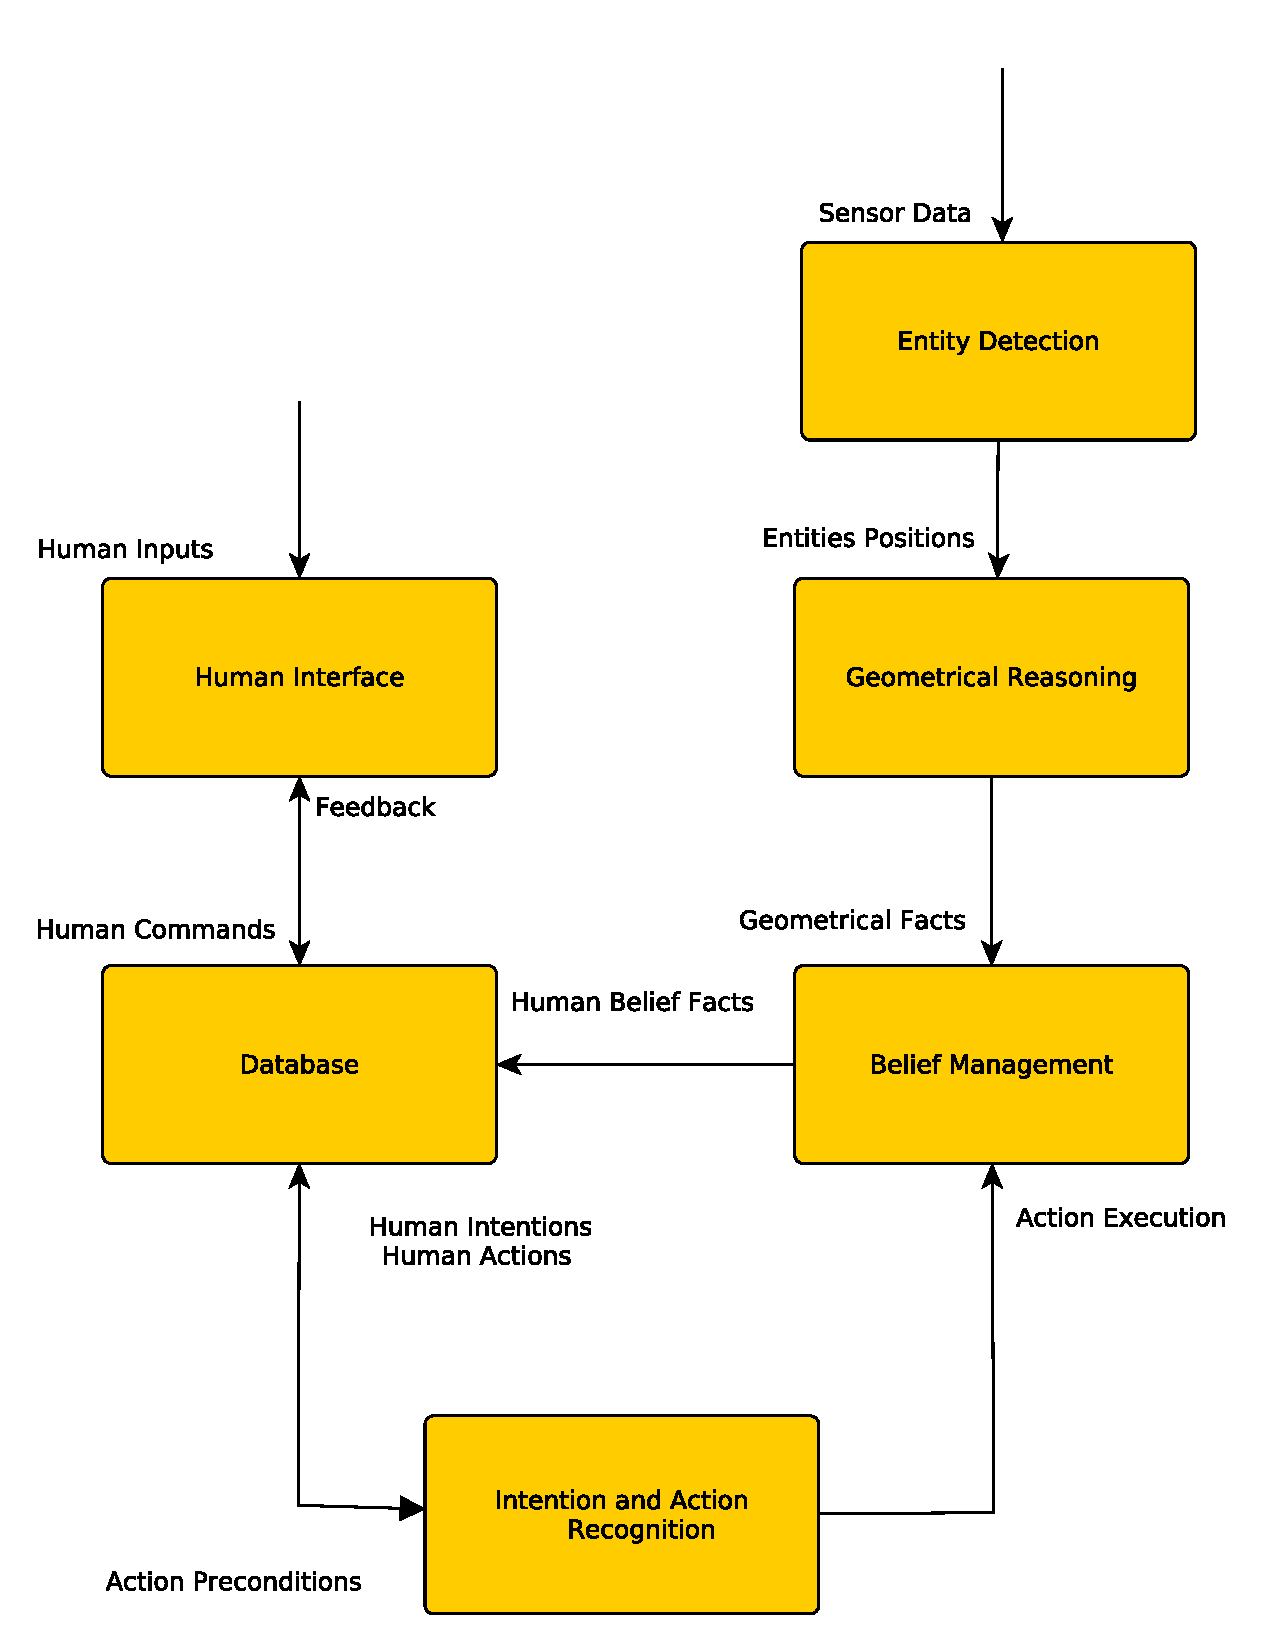
\includegraphics[scale=0.45]{img/situation_assessment/situation_assessment_overview}
	\caption{Overview of the different modules composing the Situation Assessment Layer}
	\label{fig:situation_assessment-situation_assessment_overview}
\end{figure}

In addition, the system possesses a description of the world, with a definition of all the elements known to the robot, like objects and agents, possible actions, possible intentions, intentions, etc. 
Symbolic facts are constantly produced starting from the sensor data and from the position of entities, and then the Belief Manager will update and maintain the belief model of each agent. The belief model of humans and of the robot will be used by the Intention and Action Recognition modules to infer the most likely intentions and actions performed. All these information are introduced in the Database, and can be read by other components. For example, the Goal Manager can choose a goal based on human commands or on an estimation of its intention. In a similar way, the Action Execution modules will read the Database in order to obtain the state of the world, to check action preconditions.  

Our situation assessment layer was presented in \cite{Milliez2014}, where it was used to pass the Sally and Anne test~\cite{Baron1985} on a robotic platform. The intention and action recognition capacity was introduced in \cite{devin2016some}.

\section{Object and Human Detection}
\label{sec:situation_assessment-object_human_detection}
In our system, we chose to simplify perception issues, focusing on reasoning aspects. We associate a unique tag to every object that is interesting in a particular scenario.  When the robot observes a tag using a camera, it detects the corresponding object using a tag-matching algorithm.
Regarding humans, we use a motion capture software to identify and track agents moving in the environment. Using different tags, we can track the head, shoulders, and right arm of a human. Our situation assessment component has also been tested using a laser and RGB based detector in the SPENCER european project \footnote{http://www.spencer.eu/}.


%TODO: image of MOCAP and VIMAN

\section{Human-Robot Communication}
\label{sec:situation_assessment-communication}

Similarly, communication between the human and the robot is limited, in our system. Humans can give commands to the robot by using a tablet application, where they can manage the robot goals, by adding a new goal, canceling a previous one, or pausing the robot. Requests are added to the Database, and can be read by the Goal Management Layer. The robot is able to provide simple verbal output by using a text-to-speech component. The robot is not able to perform real dialogues with the human but it can adapt its speech to the current tasks and scenarios, by explaining plans, informing the human if it has a problem, verbalizing its current actions, and so on. This feature will be explained fully in chapter \ref{chap-plan production and management}. 

%TODO: image of the tablet application

\section{World Model and Geometrical Reasoning}
\label{sec:situation_assessment-situation_assessment}
The first step in estimating human intentions is reasoning about the environment and the belief of humans. Our world is composed by agents, the robot and humans; by objects; and by areas, which are bounded regions in the environment with semantic meaning, e.g. living room, kitchen. To be more generic, we will sometimes use the word \textit{entity} to refer to an agent, an agent's joint or an object. We can assign properties, to entities and areas to represent different information, e.g. 
an agent can be in a specific area, a box can be opened and can contain objects, a bottle can contain liquids, a mug can be hot. The $subject$ of a property is the name of the primary entity linked to it (e.g. bob, mug). 
 We divide properties in two classes: 
\begin{itemize}
\item fully observable:  can be seen by any present agent looking at the linked entity or area, e.g. the box is open
\item partially observable: can be observed by present agents only in specific situations, represented as rules linked to the object and the property, e.g. an agent can see that a box contains items only when it is open, an agent can detect that the mug is hot only when he touches it.
\end{itemize}

Using its perception abilities the robot can build a representation of the environment, starting with entities' positions. Using geometrical reasoning we can compute spatial relationships between entities, e.g. the glasses are on the shelf, the human is moving toward the library, the glasses are reachable by the human, the bottle is visible for the human. These reasonings provide a base for the perspective taking abilities of the robot. 


%TODO: Image of geometrical reasoning

\section{Belief Management}
\label{sec:situation_assessment-belief_management}
In our system, agents can have divergent representations of the world. To model this aspect, the information produced by perception, geometrical reasoning and inference, are collected by the robot in \textit{belief models}, built for itself and for each agent. A \textit{belief model} is a symbolic representation of the world state, as known by an agent. In a model, the world state is represented by properties and values. To represent the lack of knowledge of an agent, the value of a property can be \textit{unknown}.

We consider our world as a dynamic environment, where properties can change and actions can be performed.  We define an action as a tuple $(name, preconditions, target, postconditions)$. The $name$ of an action is a unique string that identifies it. The $preconditions$ are a list of properties that must be true in order to realize the action. In our system, an action is executed on a $target$, which can be a physical object, like a cup, but also an area of the environment, like a room. The $postconditions$ are the set of properties, and their values, affected by the action's execution.

Since we are interested on reasoning and not perceptual aspects, we use inference, as explained in Sec. \ref{sec:situation_assessment-intention_recognition}, in order to understand when a human has performed an action. Through the predefined $postconditions$ of actions we can also infer changes in object properties, e.g. the human opens a box, so the box is now open. 

We created a rule based framework in order to build the beliefs of each agent and update them when needed. Human belief models are updated using the perspective taking skills of the robot. When the robot detects the execution of an action in the world, it updates the belief model for itself and for every human that can perceive the action, adding the action's $postconditions$ to their models. When an action is not perceived by a human (e.g. the user was in an other room), his belief model will not be updated, as he is not aware of the changes that occurred.

However, when he comes back and looks at the environment, we assign him a new belief state following a set of rules, which we will now explain. We call $H$ the agent, $HB$ his belief model, and $RB$ the robot's belief model. We also create the following predicates: $obs(p)$ means that the instance of property $p$ is observable, $valid(p,x)$ means that the instance of property $p$ doesn't contradict the current perception data of agent $x$, $value(p,m)$ is the value of predicate $p$ in belief model $m$, and $vis(p,x)$ means that agent $x$ has visibility on the linked entities of property $p$. The rules for the $valid$ predicate will be different in each property. For example the property \textit{MUG isOn TABLE} won't be valid for agent Max if he can see that there is no mug on the table. For each property $p\in HB \cup RB$:
\begin{itemize}
\item if $p \in RB, \quad p\not\in HB,\quad obs(p),\quad vis(p,H) \rightarrow value(p,HB)=value(p,RB)$.
\item if $p \not \in RB,\quad p\in HB,\quad obs(p),\quad vis(p,H) \rightarrow remove\quad $p$ \quad from \quad HB$.
\item if $p\in RB,\quad p\in HB$ then:
	\begin{itemize}
      \item if $value(p,HB)\neq value(p,RB),\\ \quad obs(p),\quad vis(p,H) \rightarrow \\ value(p,HB)=value(p,RB)$.
      \item if $value(p,HB)\neq value(p,RB),\\ \quad !obs(p),\quad !valid(p,H) \rightarrow \\ value(p,HB)=\textit{unknown}$.
	\end{itemize}
\end{itemize}
The idea of this set of rules is updating an agent's mental belief model for a property only if it's observable, or if it's not observable and perception data contradicts the current value of the property (e.g. the mug was moved from the table to the kitchen while the agent was in another room: while the agent can not see where is the mug, he can see it is no longer on the table).


%TODO: Image of perspective taking

\section{Action and Intention Inference}
\label{sec:situation_assessment-intention_recognition}

In order to infer human intentions, we will provide the following information to the robot: a list of known contexts, a list of known intentions, a list of known actions, a set of observations of human actions, and a belief model of humans and of itself.

We propose, as central model used for intention estimation, a framework based on BNs. We call our implementation of BN an Intention Graph (IG).
An IG is linked to a specific agent, and composed by the following layers of nodes:
\begin{itemize}
\item Context Nodes: these nodes represent contextual information, modeled as boolean variables (e.g. HotDay, ColdDay).
\item Intention Nodes: these boolean nodes represent the set of possible intentions. Each intention can conditionally depend on several contexts.
\item Action Nodes. This is the set of human actions whose preconditions . Each of these nodes is conditionally dependent on all the intention nodes. 
\item Observation Nodes. We associate to each action a different set of observation nodes, that depend conditionally on the associated action node. 
\end{itemize}

In a typical usage, the robot will create, for each monitored human, an IG, formed by the Context and Intention Nodes, which we consider statically known by the robot, and a variable list of Action and Observation nodes, which depends on the human's belief model. The robot will create action nodes for each known action whose $preconditions$ are satisfied in the human's belief model, and their related Observation Nodes. These IGs will need to be updated every time that an agent performs an action, switching the previous Action and Observation nodes with new ones, that will depend on the state of the world after the action was performed.

When monitoring a human, we set Context Nodes and Observation Nodes as \textit{evidence}, considering them observable by the robot. These information will allow us to have a good estimation of the most likely actions and intentions of the human, as explained in \ref{intention and action inference}.

An example of IG, taken from an experiment, can be seen in figure \ref{fig:situation_assessment-intention_graph}. In the following paragraphs, we will explain the role of these layers of nodes, and how the conditional dependencies between them are computed.

 \begin{figure}[h!]
	\centering
	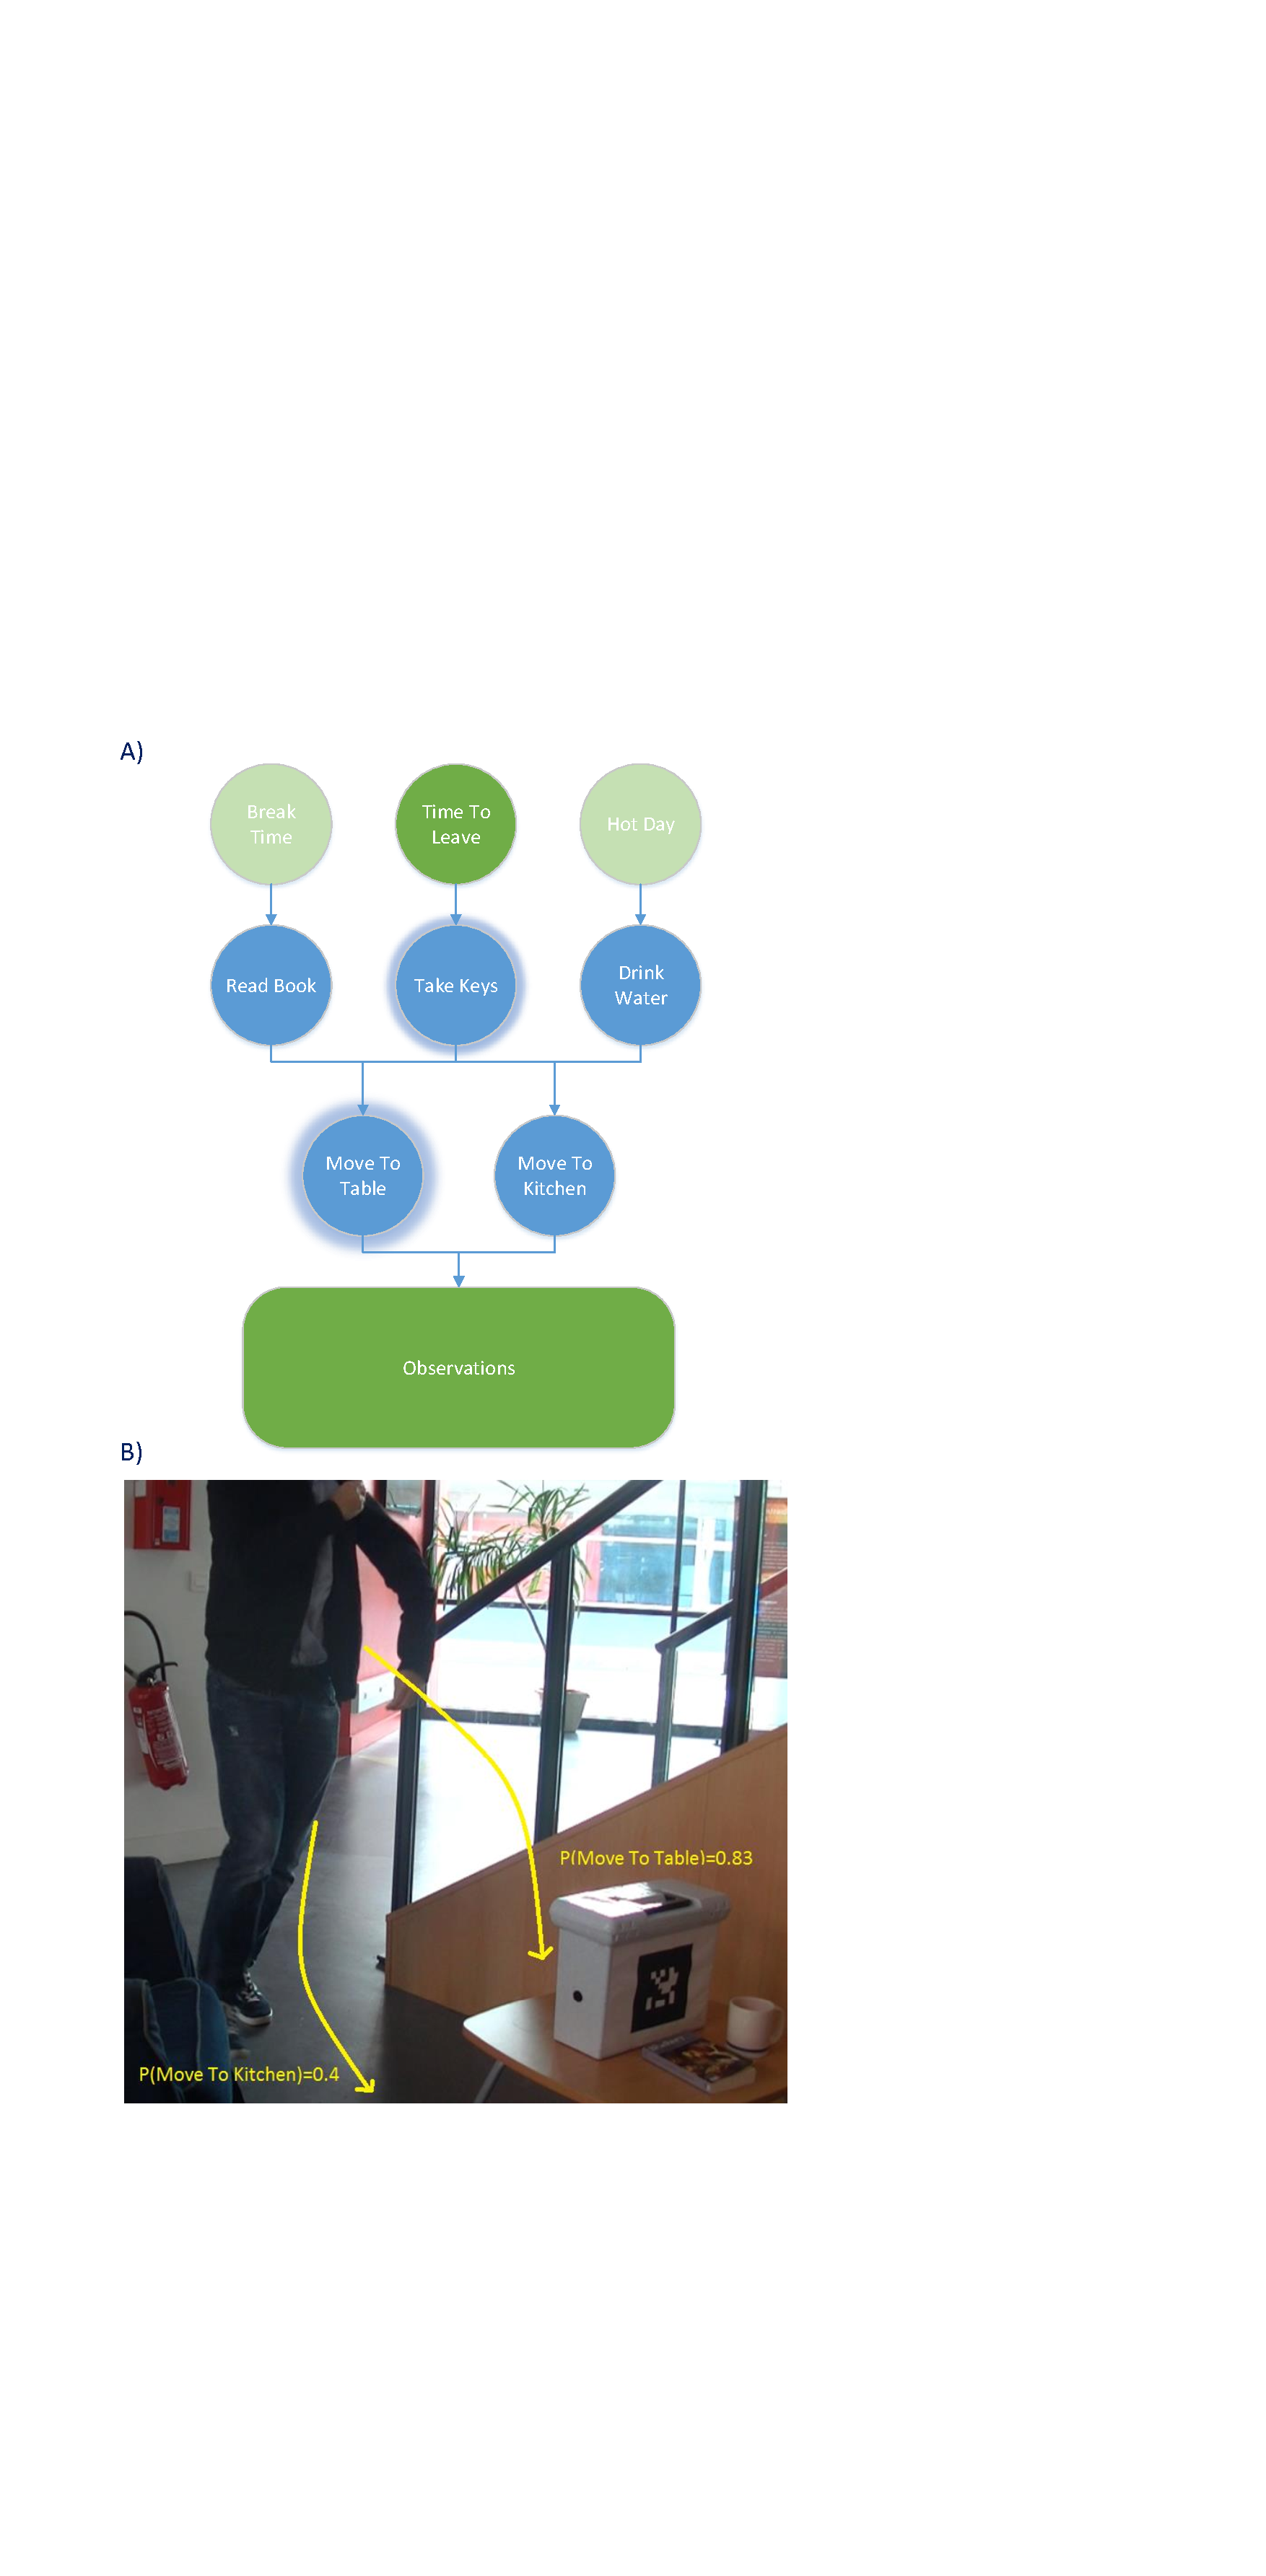
\includegraphics[trim={2cm 11cm 11cm 17cm},clip,scale=0.45]{img/situation_assessment/cookieScenario.pdf}
	\caption{A scene from our experiment. The yellow arrows show possible actions and their associated probabilities. The diagram represents the current IG. Green circles represent evidence nodes and blue circles other nodes. For the Context Nodes (top of the graph), we represented nodes with a false value as greyed out, and nodes with a true value as green. The most likely nodes in the graph are represented with a glowing effect. The observation nodes where compressed in a single block to simplify the diagram}
	\label{fig:situation_assessment-intention_graph}
\end{figure}

\subsection{From Contexts to Intentions}
We introduce a set of contexts in our domain. We consider as context any information that can be used to characterize and motivate an intention \cite{abowd1999towards}. We model a context  as a property, which can assume different values and influences the probability of a user having a particular intention. For example, we imagine that a human is more likely to be cooking at dinner time, or to drink a hot mug of tea on a cold day.

Contextual nodes can directly influence one or more Intention nodes. In this work, we chose to learn these conditional dependencies from humans, as explained in section \ref{situation_assessment-experiments}.

\subsection{From Intentions to Actions}
\label{sec:situation_assessment-action_evaluation}
To understand how actions are linked to intentions the robot needs to answer the following question: what actions would a human take, in this situation, given his belief of the world, in order to achieve its intention?
Our idea is based on the principle of rationality \cite{Dennet1989}, which states that agents tend to choose the most efficient actions, taking into account their beliefs about the world, in order to achieve their desires.

In \cite{Blakemore2001}, the authors explain that "the attribution of intentions to actions might rely on simulating the observed action and mapping it into representations of our own intention". We represent this idea by providing the robot with a set of planning models. Each one of these planning models is related to an intention, and represents all the known plans to achieve its linked goal. In this way, we can estimate how much the current human actions are compatible with the plans related to an intention.

In our implementation, for each intention known by the robot, we will create an associated Markov Decision Process (MDP), to represent all the possible plans associated to this intention. After solving the set of MDPs we will use the calculated action value function \(Q(s,a)\), to create conditional dependencies between Intention and Action nodes in the IG. Let's start by defining \(P(a|I_i=1)\), the probability that action $a$ will be performed if intention $I_i$ is true. We model this probability as \(P(a|I_i=1)=\frac{Q_i(s,a)}{\sum_b(Q_i(s,b))}\), where we normalize the value function $Q_i(s,a)$ for intention $i$ and action $a$ in the human's belief state $s$, over the value function $Q_i(s,b)$ calculated on all the monitored actions $b$. We can extend this calculation to the case where a generic number of intentions are true to compute the probabilities of action nodes: \(P(a|I_1,I_2,...,I_m)=\frac{\sum_{i:I_i=1}Q_i(s,a)}{\sum_b\sum_{i:I_i=1}Q_i(s,b)}\).

The key idea in this problem is to use the human's belief state as input for the MDPs' value functions. In this way we are using perspective taking at a planning level as the human action is consistent with his intention in his own belief state but may be irrelevant in the real world (e.g. in case of wrong belief).

Our idea is similar to \cite{karami2010human}, where human intentions are estimated using a POMDP and a set of MDPs, that simulate human policies related to different intentions. In this work we use a BN instead of a POMDP, which allows us to separate the mechanisms used for inference and for the robot's actions. Also, we improve the recognition process by including the belief state of the human.

\subsection{From Actions to Observations}
Intentions will be inferred from human actions, so the robot needs to monitor their execution. For each Action Node we define a set of four Observations Nodes: the distance of the human's body from the action's $target$, its variation, the distance of the human's hand from the action's $target$, and its variation. The conditional dependencies of the Observation Nodes are precomputed.

\subsection{Intention and Action Inference}
\label{sec:situation_assessment-intention and action inference}
We assume, in this work, that at each moment a human can only execute a single action, and the robot will react only on his most likely intention. The most likely action and intention are inferred from the BN in the following way. We call $P(n)$ the inferred probability of a node $n$, $B(n)$ the set of brothers of $n$ (that is, nodes on the same layer), and $\delta_1$, $\delta_2$ two thresholds. The robot infers that an action has been realized, or that a human has an intention following these rules: 
\begin{itemize}
\item  \(P(n_i)>\delta_1\) 
\item  \(\forall b \in B(n_i): P(n_i)>P(b)+\delta_2\), where $n_i$ is the node associated to the interested intention or action.
\end{itemize}

When the robot infers that an action has been performed, it updates the world state with its $postconditions$, triggering an update on the beliefs of all present agents. The current human intention is recorded in the Database, in order to be used by the Goal Manager.

\subsection{Proactive Behaviors}
\label{subsec:situation_assessment-proactive_behaviors}
Information about the most likely intention and action will be introduced in the database, to be read by the Goal Management module. Based on this information, the robot can execute two different proactive behaviors: correcting the belief state of the human, and proactively helping him to achieve his task.

\subsubsection{Correcting Belief State}
Having a wrong or incomplete belief on the world state can lead agents to execute non optimal, useless, or even dangerous actions. The robot needs to detect these situations in order to warn the human. The robot assumes that it always holds a correct belief state. Our solution uses the expected action rewards introduced in \ref{sec:situation_assessment-action_evaluation}. The idea is comparing the expected reward for performing an action according to the human and the robot's belief states. To formalize: we compare the action values \(Q_m(s_h,a_h)\) and \(Q_m(s_r,a_h)\), where $m$ is the most likely intention,  $s_h$ and $s_r$ are the robot's and human's belief state, and $a_h$ is the most likely action. If these values are not equal the human expects a different outcome from its action than what should actually happen. 

We propose a simple solution, where the robot warns the human of the detected divergent belief for that action. For example, Bob wants to drink tea from a closed, opaque bottle, which the robot knows is empty (perhaps because another agent drank the last glass), while Bob does not. When he approaches the bottle, the robot detects that his most likely intention (using the process described in \ref{sec:situation_assessment-intention_recognition}) is to drink tea. The system calculates the expected rewards from taking the bottle in the two belief models and obtains different values. The system checks the property values associated to the bottle in the two mental models, and extracts the differences. Using this information, the robot corrects the divergent belief, informing the human that the bottle is now empty. 

To implement this idea, in our system, detecting the need to correct a belief state, the Intention and Action Recognition module will introduce all the needed information in the Database, which will be read by the Goal Manager in the form of a "warn agent" goal with high priority (as will be explained in chapter \ref{chapter-goal_management}).

\subsubsection{Performing a part of the plan}
There are situations in which the robot should help the human achieve its goal by acting. The Goal Management layer will consider new inferred intentions as possible goals for the robot, and will communicate with the Plan Production and Management layer to achieve them, as explained in chapters \ref{chapter-goal_management}, \ref{chapter-plan_management}, and \ref{chapter-plan_execution}. 


\section{Experiments and Discussion}
\label{sec:situation_assessment-experiments}
\subsection{Case Study}
Evaluating the capacity of the system to estimate human intentions is not easy, since intentions are not directly observable. A possible solution, as shown in \cite{baker2014modeling}, is comparing the estimation of human intentions, performed by other humans, with the predictions of our system. In order to perform this comparison we created a user study where we showed participants several videos, asking them to estimate the likelihood of a set of intentions for each video, and collected their results. 

We performed an equivalence test, comparing users' intentions predictions with those of the robot, following the two one-sided tests (TOST) approach. We choose as a threshold for equivalence the standard deviation $\sigma$ of the users' answers. The idea behind this choice is that, if the robot's answers are closer than a standard deviation to the average human answers, its predictions are comparable to an average human answer from our user group. 

We defined our hypothesis as follow: 
\begin{itemize}
\item $H_0$: $\mu_{hi}-\mu_{ri}\leq-\sigma_{hi}$ OR $\mu_{hi}-\mu_{ri}\geq\sigma_{hi}$ 
\item $H_A$: $-\sigma_{hi}<\mu_{hi}-\mu_{ri}<\sigma_{hi}$  
\end{itemize}
where $\mu_{hi}$ and $\mu_{ri}$ are the human average and the robot's answer for test $i$, $\sigma_{hi}$ is the variance of the human answers for test $i$.

We performed tests to evaluate: a) prediction in absence of clues, b) prediction in the presence of contextual clues, c) prediction in the presence of belief state clues.

We built a household environment with a fixed set of furniture: a \textit{Kitchen Shelf}, a \textit{Table}, a \textit{Sofa}, and a \textit{Chair}. In this environment, we created two scenarios, composed by several tests, with two agents, \textit{Max} and \textit{Bob}, performing different actions. Each scenario contained a set of objects, and a constrained set of intentions. For the tests related to belief states, we start by showing the users and the robot a specific sequence of events, allowing them to build a mental model of the agents. We will describe in details the two scenarios and the relative tests.

\subsubsection{Cookie Scenario}
\begin{itemize}
\item Objects: a \textit{Cookie Box}, a \textit{Mug}, and a \textit{Bottle of Water} were placed on the \textit{Table}, close to each other. A pack of \textit{Cookies} was placed on the \textit{Kitchen Shelf}. The \textit{Cookie Box} could contain, or not, \textit{Cookies}.
\item Intentions: \textit{Eating a Cookie}, \textit{Drinking Water}, \textit{Reading the Book}.
\item Tests:
\begin{itemize}
	\item \textit{No Clues}: \textit{Max} approaches the \textit{Table}.
    \item \textit{Contextual Clues}: \textit{Max} approaches the \textit{Table} commenting on the warmth of the day.
	\item \textit{Divergent Belief Max}: \textit{Max} approaches the \textit{Table}.
	\item \textit{Divergent Belief Bob}: \textit{Bob} approaches the \textit{Table}.
\end{itemize}
\item  \textit{Divergent Belief Event}:  \textit{Max} and \textit{Bob} are chatting on the \textit{Sofa}. Max eats the last \textit{Cookie} from the \textit{Cookie Box} before closing it and leaving. While \textit{Max} is away, \textit{Bob} takes \textit{Cookies} from the \textit{Kitchen Shelf}, fills the \textit{Cookie Box} with them, and closes it, before leaving.
\end{itemize}

The \textit{Divergent Belief Event} was shown to the users and the robot between the \textit{Contextual Clues} and the \textit{Divergent Belief Max} events. 

We deliberately included an intention, \textit{Reading the Book}, without placing a book in the visible environment, introducing a confusing element in the scenario.

\subsubsection{Keys Scenario}
\begin{itemize}
\item Objects: A \textit{Box} was placed on the \textit{Table}, that partially occluded the sight of people approaching. A \textit{Book} and a \textit{Mug} where placed behind the \textit{Box}, so that they could be seen from the sofa but not from approaching people.
\item Intentions: \textit{Taking the Mug}, \textit{Taking the Keys}, \textit{Reading the Book}.
\item Tests and Events:
\begin{itemize}
\item \textit{No Clues}: \textit{Max} approaches the \textit{Table}.
\item\textit{Contextual Clues}: \textit{Max} approaches the \textit{Table} in a hurry, while putting on a coat.
\item \textit{Divergent Belief Max}: \textit{Max} approaches the \textit{Table} in a hurry, while putting on a coat.
\end{itemize}
\item \textit{Divergent Belief Event}: \textit{Max} is sitting on the \textit{Table}, drinking from the \textit{Mug}, while having the \textit{Keys} in his hands. His phone rings, so he drops the \textit{Keys} and the \textit{Mug} on the \textit{Table}, behind the \textit{Box}, and leaves the room. While \textit{Max} is away, \textit{Bob} comes and sits on the \textit{Sofa}, reading a \textit{Book}. When he sees the \textit{Keys}, he takes them, places the \textit{Book} on the \textit{Table}, and leaves.
\end{itemize}

The \textit{Divergent Belief Event} was shown to the users and the robot between \textit{Contextual Clues} and the \textit{Divegent Belief Max} events.

\subsection{User Study}
We built an online user study, where we presented videos related to the tests and events of the two scenarios to users, who had to evaluate the likelihood of each intentions of the scenario
on a five-level Likert scale. The user study was conducted in three languages, with users living in two different countries\footnote{A version of this user study was provided at http://goo.gl/forms/YiuFHnF63c}. We collected answers from 78 adults, performed an average, and converted them to percentile scores, in order to compare them with the robot's predictions.

Looking at users' answers (Fig. \ref{fig:situation_assessment-user_study_results}), we can see that, in the absence of clues, people rated similarly the two intentions related to visible objects. Contextual clues had the highest influence on users' ratings. This is particularly visible in the \textit{Contextual Clues} test of the \textit{Keys Scenario}, where users chose as the most likely intention \textit{Take Keys}, even if no keys were visible in the video. Divergent beliefs also influenced users decisions, but not as strongly as context. The strongest responses, over all, where given by the \textit{Divergent Belief Max} test on \textit{Keys Scenario}, which uses both divergent belief and contextual information.

\subsection{Robot implementation}
At the start of a scenario the robot scanned the environment, building a model of its world state. With our perception capacities, we can't detect if the cookie box is full or empty, and so we consider it as full at the start of a test, and update its value using the $postconditions$ of inferred human actions. We consider the box as empty when we infer that a human has taken a cookie from inside, and as full when we infer that a human has put a cookie in it.

We built different IGs for the scenarios. Each test had a different graph, related to it's main agent. We considered three different Context Nodes for these IGs: Hot Day, true when the day is particularly warm; Break Time, true when the agents are taking a pause; Time to Leave, true when it's late in the day, and the humans usually leave work and return home.

As previously said, we chose to follow \cite{Liu2014} in order to learn the link between Contexts and Intentions. We created a second user study with 15 users, in which we presented a set of 5 scenarios, each one related to one of the intentions of our tests. For each scenario we asked the users to rate the perceived link, on a five-level Likert scale, between the intention and our three contexts. We averaged users' answers and calculated the conditional probabilities between context nodes and intention nodes from these averages.


In the \textit{Cookie Scenario} the graph for the tests is constructed from the following nodes:
\begin{itemize}
\item Context Nodes: \textit{Hot Day}, \textit{Break Time}, \textit{Time to Leave}
\item Intention Nodes: \textit{Fill Cookie Box}, \textit{Eat Cookie}, \textit{Drink Water}, \textit{Read Book}.
\item Action Nodes: \textit{Move to Table}, \textit{Move to Kitchen}.
\item Observation Nodes: distance of the agent body and hand to each action's associated \textit{interesting points}.
\end{itemize}

We introduce the \textit{Fill Cookie Box} intention, not present in the human test, to allow the robot to detect when Bob fills the \textit{Cookie Box} during the \textit{Divergent Belief Event}.

Our robot doesn't have speech recognition capacities. We simulated this capacities, and set Context Nodes to plausible values, that could be extracted by watching the videos. For the \textit{Contextual Clues} test, we set the value of \textit{Hot Day} to true (since Max is commenting about the temperature), and \textit{Break Time}, and \textit{Time to Leave} to false (since no data in the video points to one of these contexts being true. Max and Bob seem to have taken a break from work before the other events are shown, in the Divergent Belief Event).
%Our robot doesn't have speech recognition capacities. and for \textit{Contextual Clues} test, set the value of \textit{Hot Day} to \textit{true}, and the value of \textit{Break Time} to \textit{false}, i.e. the robot knows that it is not the usual time for the agents to take a break.

\textit{Divergent Belief Event}, \textit{Divergent Belief Max}, and \textit{Divergent Belief Bob} were showed sequentially to the robot, which updated the agents' mental models and created new IGs accordingly. During the \textit{Divergent Belief Event} several IGs need to be created with different action and observation nodes, to follow the sequence of actions by the two agents. For example, when \textit{Max} leaves the room, \textit{Bob} has the possibility to execute the actions \textit{Take Mug}, \textit{Take Water Bottle}, \textit{Open Cookie Box}, \textit{Move to Kitchen Shelf} or \textit{Leave Room}. Intention and Context nodes remains the same in all the IGs of the scenario.


The \textit{Keys Scenario} has a similar IG, with the following differences.
\begin{itemize}
\item Context Nodes: \textit{Hot Day}, \textit{Break Time} and \textit{Time to Leave}.
\item Intention Nodes: \textit{Drink Water}, \textit{Take Keys}, \textit{Read Book}.
\end{itemize}

Action Nodes and Observation Nodes are the same as the previous scenario, and follow the same ideas during the \textit{Divergent Belief Event}. An example of IG used in the tests can be seen in Fig. \ref{fig:situation_assessment-intention_graph}. For the \textit{Contextual Clues} and \textit{Divergent Belief} test, we set the \textit{Time to Leave} context value to \textit{true} (since Max is putting a coat and seems in a hurry), and other context node values to \textit{false}. Using the component described in the previous sections, and these IGs the robot was able to obtain predictions from the user actions.

\subsection{Discussion}
\label{sec:discussion}
We performed TOST tests for each intention in the scenarios, comparing the humans' answers with the robot's, for a total of 21 tests.

We calculated p-values and performed our tests using a significance value $\alpha=0.05$.

Analyzing the results of our equivalence tests, shown in Fig. \ref{fig:situation_assessment-user_study_results}, produces some interesting information. 1) The behavior of our system is often close to human capacities. 19 tests out of 21 passed our requirements for significance level, often with very low p-value scores. 2) Context and Divergent Belief are necessary. A system without these skills would only have been able to model properly the \textit{No Clues} cases. 3) There are still some missing aspects in our system. We failed to reject the null hypothesis for two tests. In \textit{Divergent Belief Bob} users rated higher the \textit{Eat Cookie} intention than the \textit{Drink Water} intention, possibly because they thought that since \textit{Bob} filled the \textit{Cookie Box} he may want to eat a \textit{Cookie}. This makes us think that humans use deep temporal reasoning to evaluate intentions, considering the whole history of actions performed by agents.  

 \begin{figure}[h!]
	\centering
	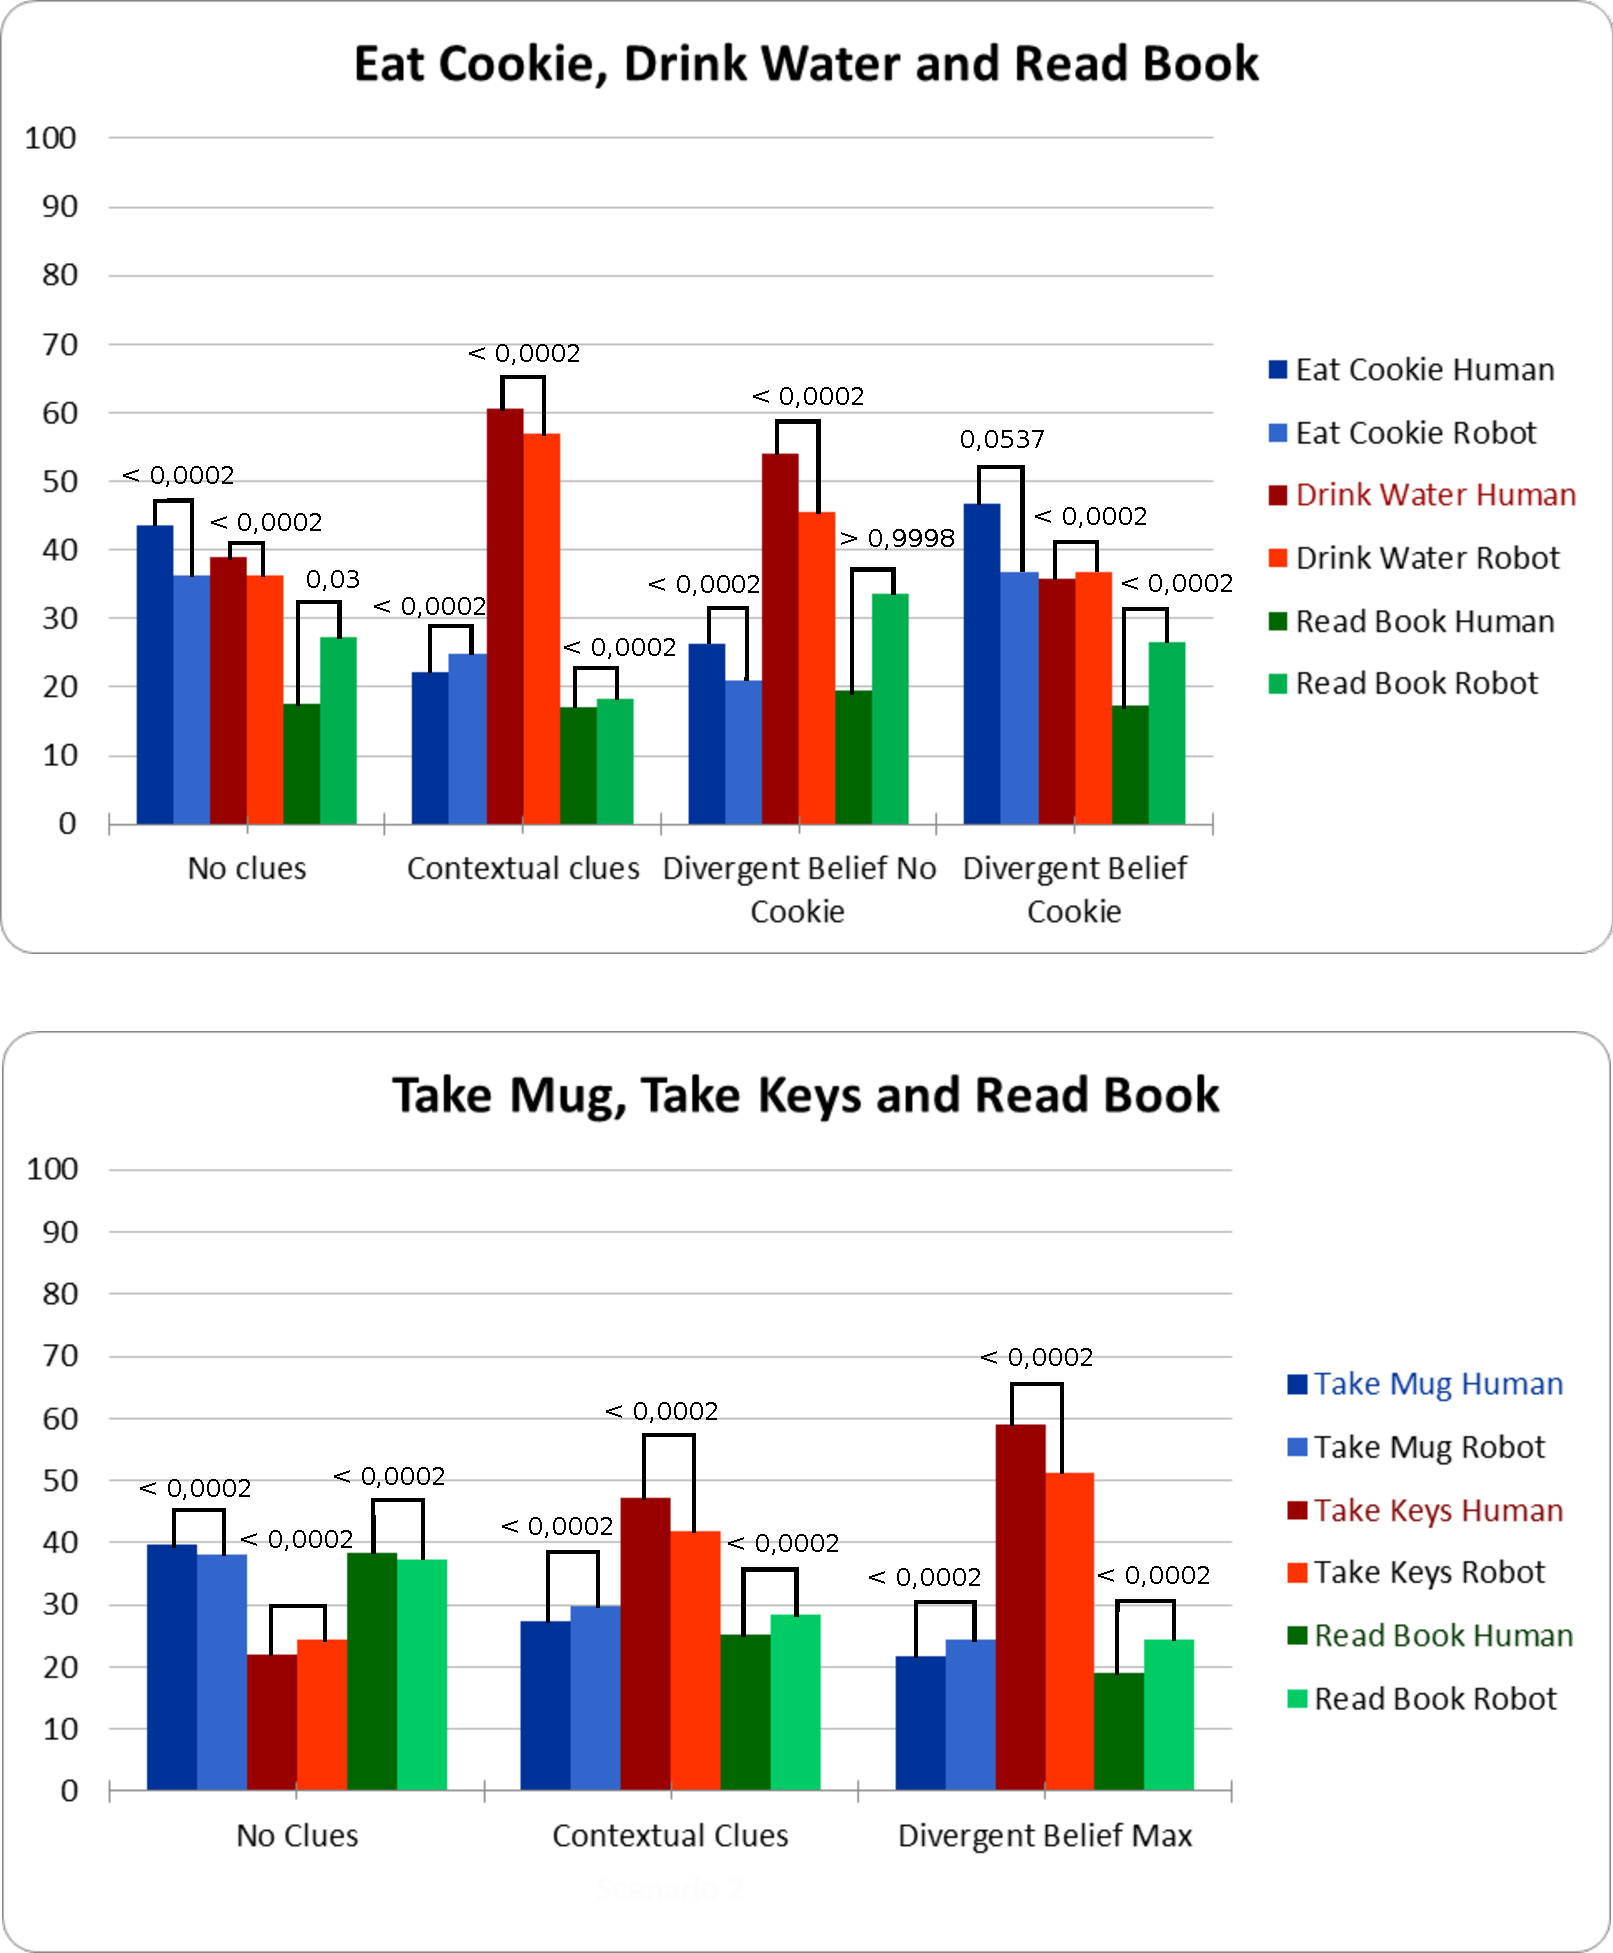
\includegraphics[clip,scale=0.32]{img/situation_assessment/pvalues1.pdf}
	\caption{Experiment results. Results from the two scenarios are represented as graphs. Intentions, as estimated by the humans and the robot, are represented by different colors, as shown in the legend of the graphs, with estimations of the same intention by the robot or the human placed in adjacent position. Each column represents the likelihood of an intention, expressed as a percentile score. P-values from the equivalence tests are shown, linking the estimation of an intention by the humans and by the robot.}
	\label{fig:situation_assessment-user_study_results}
\end{figure}



